\documentclass[letterpaper,10pt,twoside,twocolumn,openany]{book}
\usepackage[bg=full]{dnd} % this has to come first in order for this to work
\usepackage{listings}
\usepackage[english]{babel}
\usepackage[utf8]{inputenc}
\usepackage{graphicx}
\usepackage{mathtools}
\usepackage{amsmath}
\usepackage{amsfonts}
\usepackage{lmodern}
\usepackage{wallpaper}
\usepackage{tikz}
\usepackage[hidelinks]{hyperref}
\usepackage[]{dndnotes}
\graphicspath{{PDF/}{../PDF/}{../assets/}{./assets/}}
\setcounter{tocdepth}{2}

 
\usepackage{subfiles}
\colorlet{tablecolor}{PhbLightCyan}
 
\lstset{% 
  basicstyle=\ttfamily,
  language=[LaTeX]{TeX},
}


\parindent0pt  \parskip10pt             % make block paragraphs
\raggedright                            % do not right justify

% Note that book class by default is formatted to be printed back-to-back.
\begin{document}                        % End of preamble, start of text.

\frontmatter                            % only in book class (roman page #s)


\begin{titlepage}
    \begin{center}
      \begin{tikzpicture}[remember picture,overlay]
        \node[inner sep=0pt] at (current page.center) {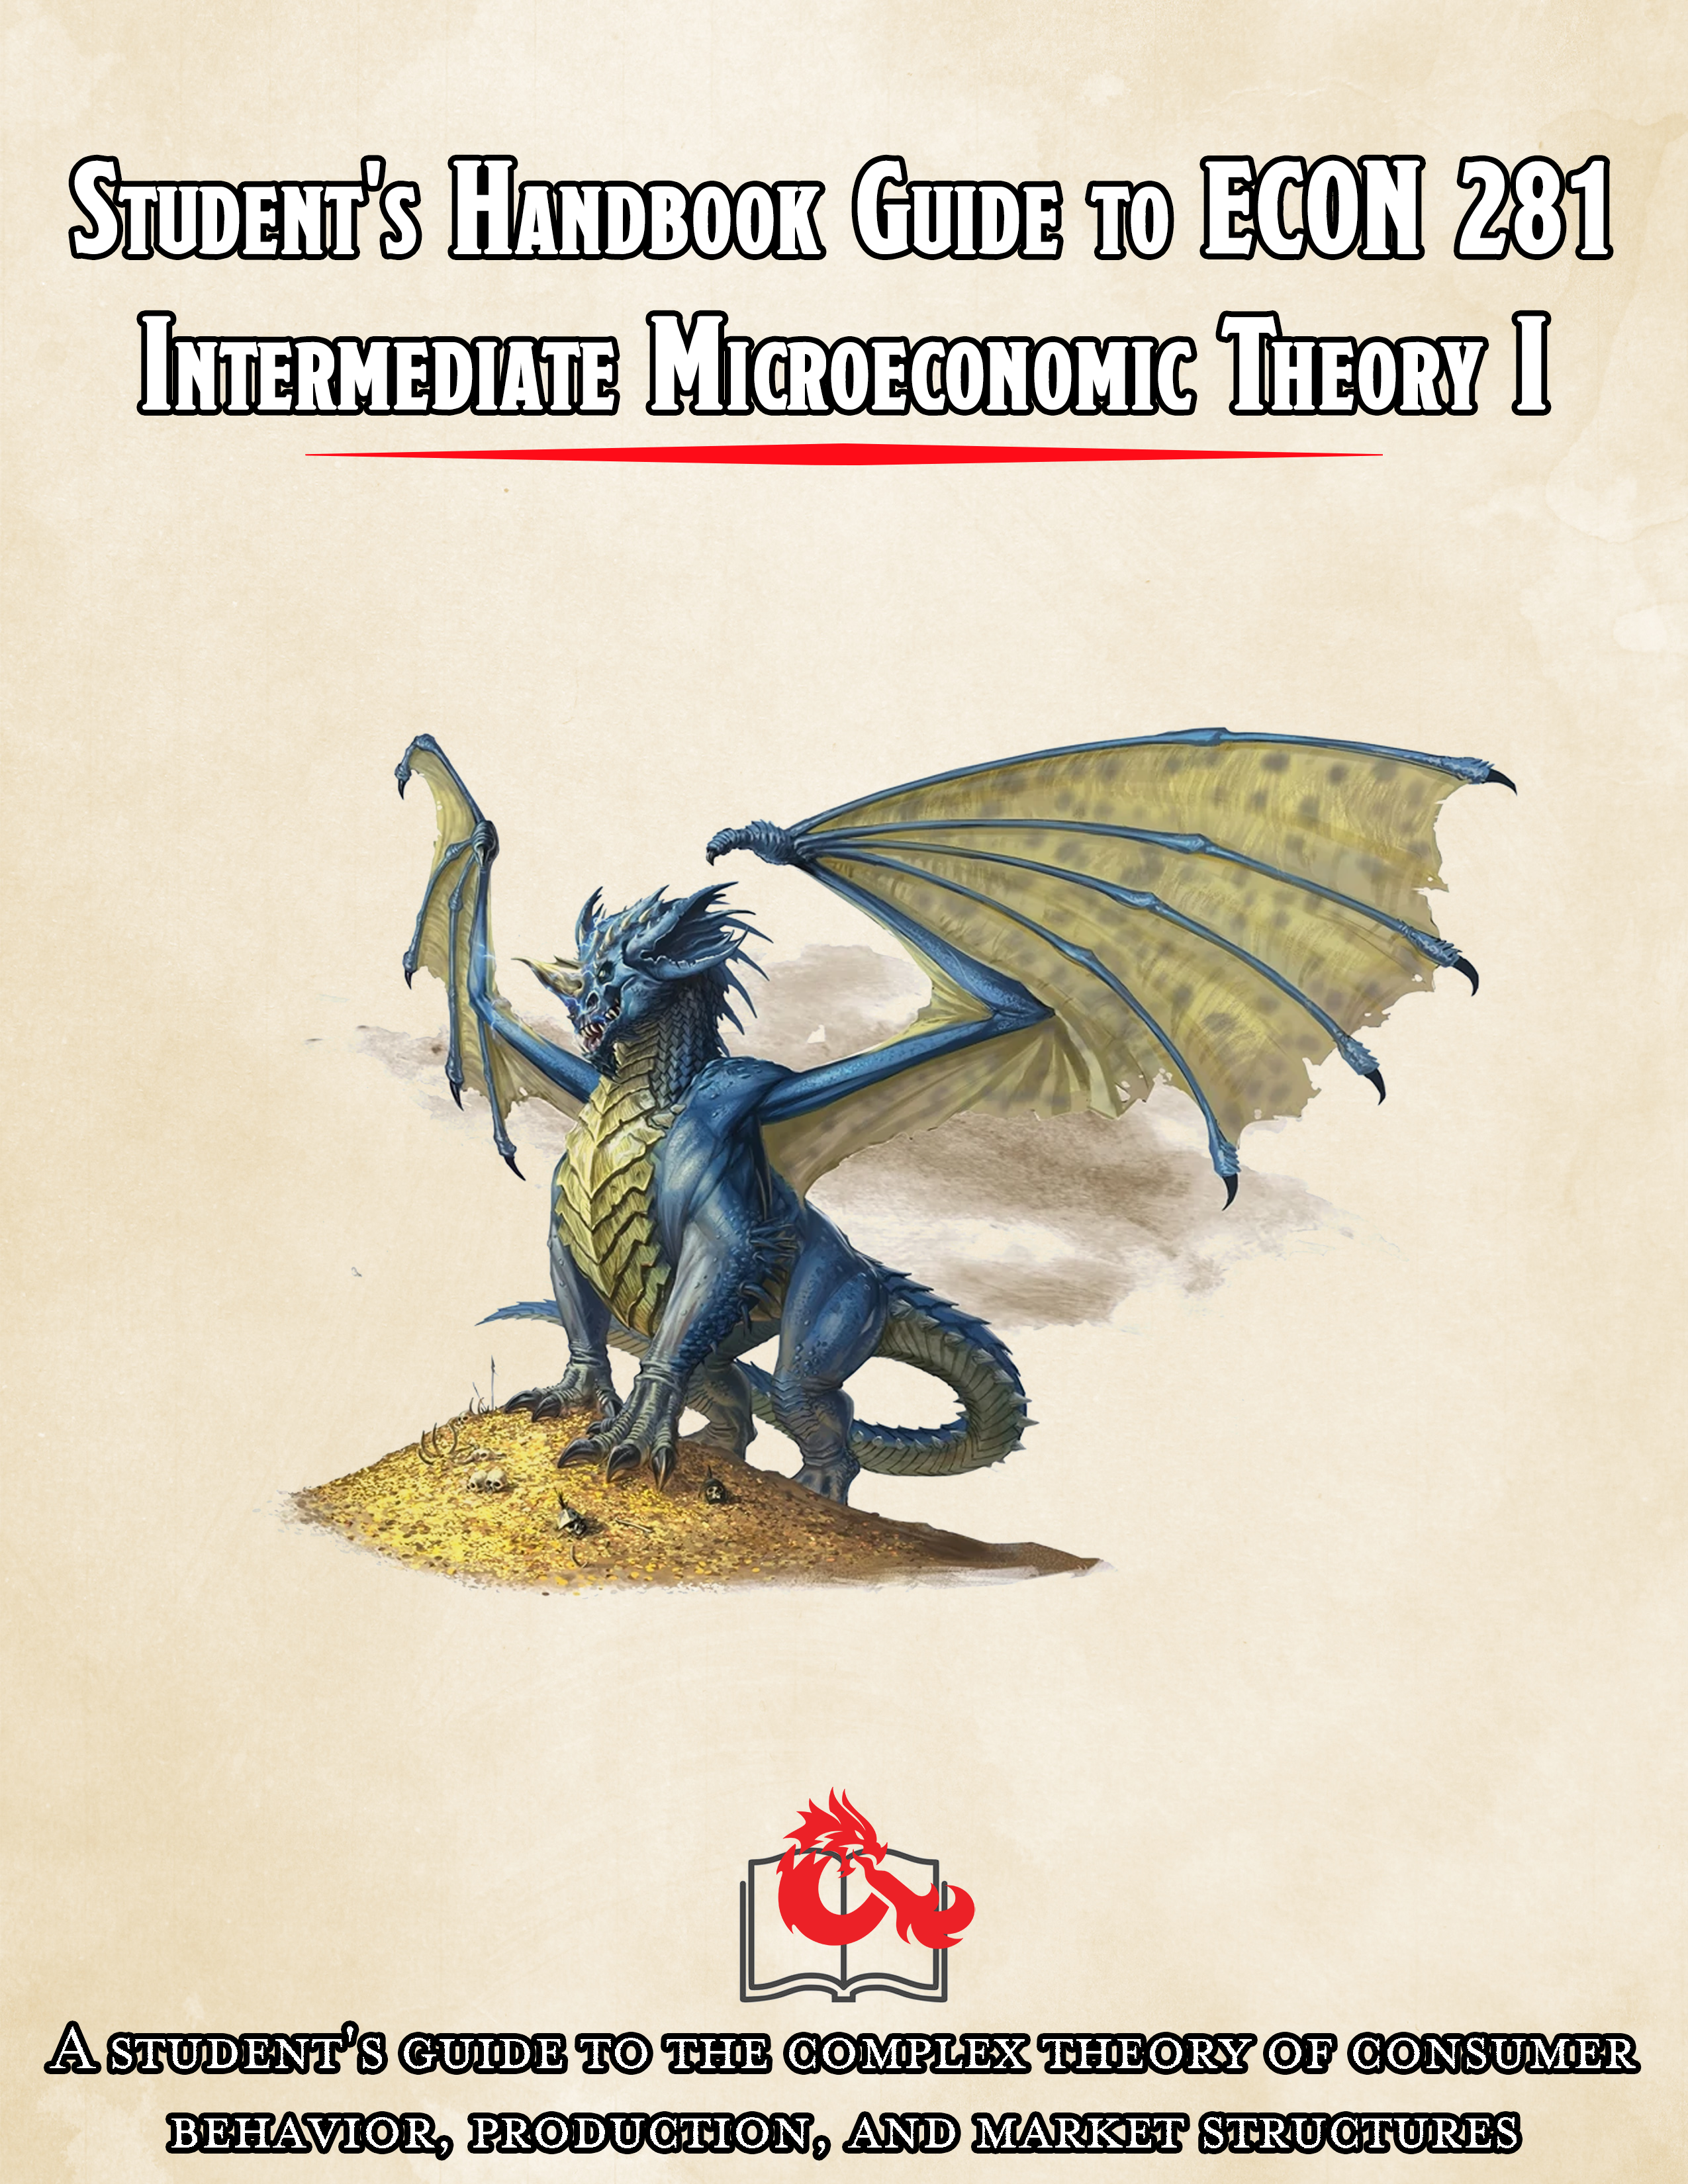
\includegraphics[width=\paperwidth,height=\paperheight]{ECON-281-Cover.png}};
      \end{tikzpicture}~      
        \newpage
        %\CenterWallPaper{1}{../paper.jpg}

        \large
        \vspace*{\fill}
        The theory of consumer behavior; theory of production and cost; price and output determination under competition, monopoly and other market structures.
        \vspace*{\fill}

    \end{center}
    \let\thefootnote\relax\footnote{Disclaimer: The following information does not contain any knowledge on how a Red Dragon grows and maintain its horde. One can consider their tactics of slavery, tyrannical governance, elimination of rivals, terrorism, or anything a dick would do to be a valid guess. However, in order to avoid being roasted by Bahamut this information will not be discussed any further.}
 \end{titlepage} 


\tableofcontents                        % Print table of contents
\mainmatter                             % only in book class (arabic page #s)
\chapter{Introduction}
We get it you like money.

\subfile{chapters/chapter2.tex}
\subfile{chapters/chapter3.tex}
\subfile{chapters/chapter4.tex}
\subfile{chapters/chapter5.tex}
\subfile{chapters/chapter6.tex}
\subfile{chapters/chapter7.tex}
\subfile{chapters/chapter8.tex}
\subfile{chapters/chapter9.tex}
\subfile{chapters/chapter10.tex}
\subfile{chapters/chapter11.tex}
\subfile{chapters/chapter12.tex}
\subfile{chapters/eval.tex}

\chapter{Credits}
\subsection{General}
\begin{itemize}
    \item Created by u\textbackslash DnD\_Notes, March 2019
    \item Typesetting engine: \href{https://www.latex-project.org/}{\textcolor{blue}{\LaTeX}}
    \item Dungeon and Dragon (5e) LaTeX \href{https://github.com/rpgtex/DND-5e-LaTeX-Template}{\textcolor{blue}{Template}}
\end{itemize}

\subsection{Art}
\begin{itemize}
    \item The Blue Dragon for the cover art is from \href{https://www.dndbeyond.com/}{\textcolor{blue}{D\&D Beyond}}
    \item Andy the D\&D Ampersand is from \href{https://www.dnd.wizards.com}{\textcolor{blue}{Dungeon and Dragons}} 
    \item Cover art formatting: Photoshop CC 2019
\end{itemize}
\subsection{Disclaimer}
This document is completely unofficial and in no way endorsed by Wizards of the Coast. All associated marks, names, races, race insignia characters, locations, illustrations and images from Dungeon and Dragon world are either \textregistered, \textcopyright, TM and/or Copyright Wizards of the Coast Ltd 2012-2018. All used without permission. No challenge to their status intended. All Rights Reserved to their respective owners.
\end{document}
